\documentclass{beamer}
\bibliographystyle{amsalpha}
\usepackage{cite}
\usepackage[normalem]{ulem}
\usepackage{fancybox}
\usepackage{enumitem}
\setitemize{label=\usebeamerfont*{itemize item}
\usebeamercolor[fg]{itemize item}
  \usebeamertemplate{itemize item}}
\setbeamertemplate{footline}[frame number]{}
\setbeamertemplate{navigation symbols}{}
\graphicspath{{figures/}}

\title{The Heterogeneous Multiscale Method}
\subtitle{Combining Molecular Dynamics with Kinetic Theory}
\author[Price and Shohet]{Jake Price}
\institute[CPSSW]{Computational Physics Student Summer Workshop}
\date{\today}

\begin{document}
	\begin{frame}
		\titlepage
	\end{frame}
	
%	\begin{frame}[t]{Outline}
%		\tableofcontents
%	\end{frame}
	
	
	\section{Multiscale Overview}
	\subsection{Overview}
	
	
	
	
	\section{Heterogeneous Multiscale Method (HMM)}
	\subsection{Overview}
	\begin{frame}{What is the Heterogeneous Multiscale Method (HMM)?}
		\vspace{1em}
		\em``HMM is a framework for linking models at different scales. It follows a top-down strategy: The basic starting point is an incomplete macroscale model, with the microscale model used as a supplement. It consists of two main components: The macroscale solver and a procedure for estimating the missing numerical data from the microscale model."\hfill\\\hfill\normalfont -Weinan E, et al, 2006
		\vspace{-1em}
		\begin{center}
			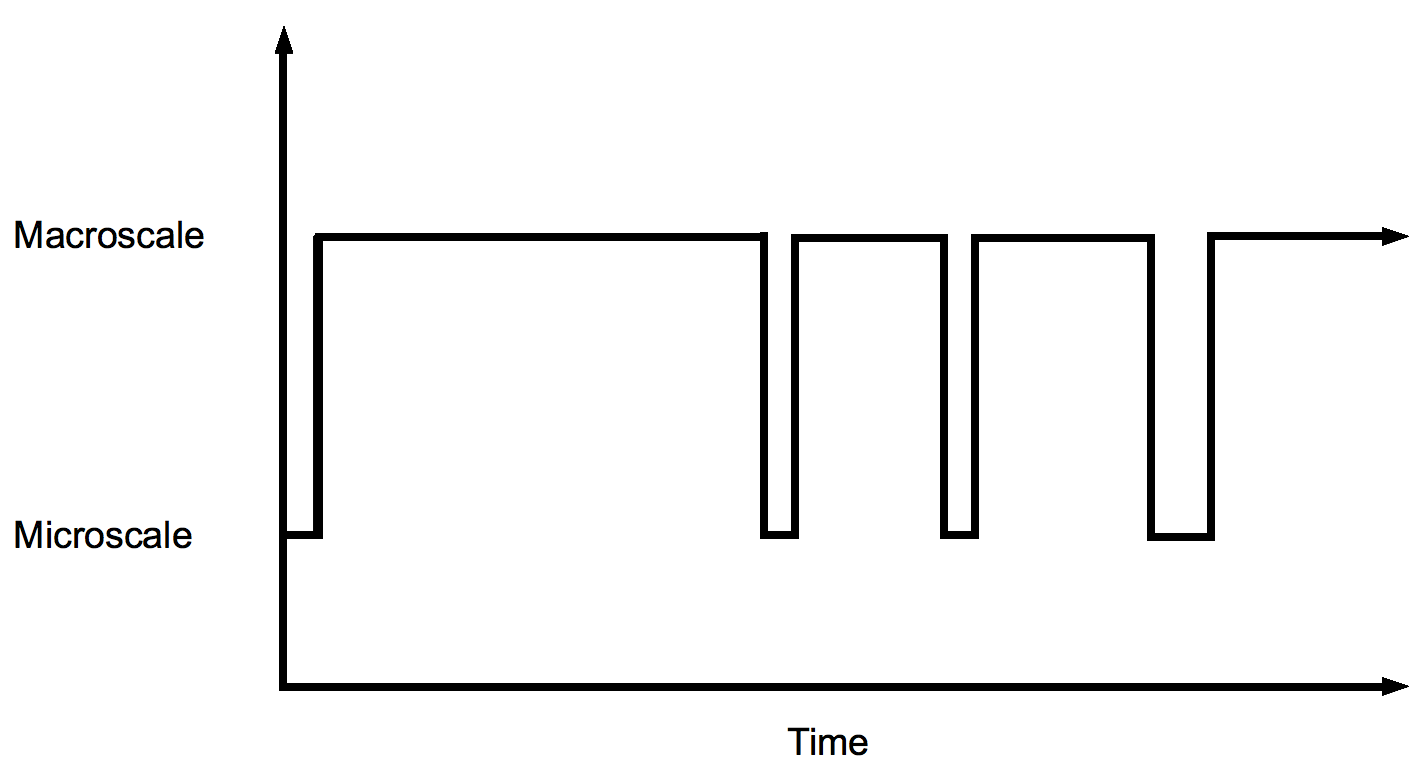
\includegraphics[height = 0.5\textheight]{scheme.png}
			\end{center}
	\end{frame}
	
	\begin{frame}{HMM Structure}
		\begin{itemize}
			\item  A \emph{compression} operator, $Q$, maps information from the microscale state to the macroscale
			\item  A \emph{reconstruction} operator, $R$, reconstructs the microscale model using the macroscale state
		\end{itemize}
		\begin{center}
			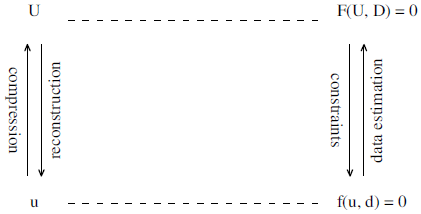
\includegraphics[width=0.7\textwidth]{framework.png}
			\\\tiny HMM Framework (Weinan E et al, 2006)
		\end{center}
	\end{frame}
	
	\begin{frame}{Types of Problems}
		\begin{enumerate}[leftmargin=1.75cm]
			\item[\textbf{Type A:}] Microscopic model is only required near isolated defects or singularities in the domain
			\vspace{1em}
			\item[\textbf{Type B:}] A nearly closed macroscale model exists but is not sufficiently explicit. The microscale model closes the system and provides missing information
			\vspace{1em}
			\item[\textbf{Type C:}] Problems with features of both \emph{Type A} and \emph{Type B} problems
			\vspace{1em}
			\item[\textbf{Type D:}] Problems that exhibit self-similarity
		\end{enumerate}
	\end{frame}
	

	

	
	
	
	\section{HMM for Plasma Modeling}
	\subsection{Problem Statement}
	\begin{frame}{My Summer Research}
		\begin{itemize}
			\item  Develop a proof-of-concept computational framework to model plasmas using HMM\vspace{1em}
			\begin{itemize}
			\item  We developed the framework to solve problems using this combination of models\vspace{1em}
			\end{itemize}
			\item  Macroscopic model: Kinetic theory using the BGK approximation of the Boltzmann equation (BGK)\vspace{1em}
			\item  Microscopic model: Molecular dynamics (MD)\vspace{1em}
			\item This is doubly novel research, because HMM has to our knowledge never been used in a plasma setting, nor has it been used with kinetic theory
		\end{itemize}
	\end{frame}
	
	\begin{frame}{Problem Statement}
		\begin{itemize}
			\item  Ions live in a three-dimensional periodic domain and are initialized such that their distribution is $x$-dependent, but uniform in $y$ and $z$
			\vspace{0.5em}
			\begin{itemize}
				\item Use statistical data from a 3D-3V MD microscale simulation to increase the accuracy of a 1D-3V BGK macroscale distribution function
				\vspace{0.5em}
				\item  May have $n$ species with different masses and charges
				\vspace{0.5em}
			\end{itemize}
			\vspace{0.5em}
			\item  The mathematical framework is built up from first principles and designed to be as general as possible
			\vspace{0.5em}
			\item  \emph{Type B} problem: we are using the MD to close our macroscale kinetic model
		\end{itemize}
	\end{frame}
	
	\subsection{Model Formulation}
	\begin{frame}{Model Choices}
		\begin{center}
			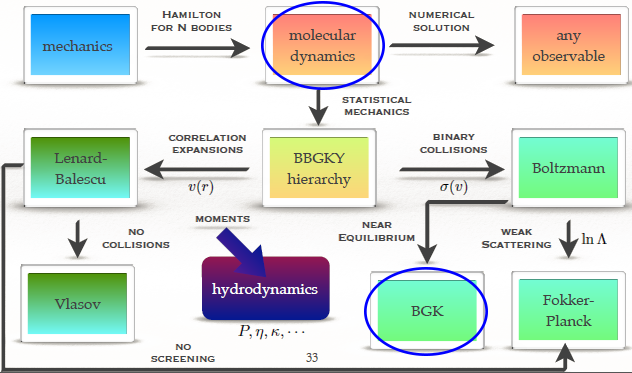
\includegraphics[width=1\textwidth]{KT_structure.png}
			\\\tiny Structure of kinetic theory models (Murillo, 2015)
		\end{center}
		
	\end{frame}
	
	%\begin{frame}{Model Formulation}
%		\begin{itemize}
%			\item  The models are derived from a Klimontovich distribution of $N$ particles, $\phi_k$, that stores the location, $\mathbf{r}_i$, and velocity, $\mathbf{v}_i$, of each ion $i$ of each species $k$ at a given time $t$:
%			\begin{equation*}
%				\phi_k(\mathbf{r},\mathbf{v},\{\mathbf{r}_\alpha\}_{\alpha=1}^{N},\{\mathbf{v}_\alpha\}_{\alpha=1}^{N},t) = \sum_{i\in S_k}\delta\left(\mathbf{r}-\mathbf{r}_i(t)\right)\delta\left(\mathbf{v}-\mathbf{v}_i(t)\right).
%			\end{equation*}
%			\vspace{0.5em}
%			\item  To preserve generality, we formulate our equations in a dimensionless form using a set of plasma parameters and arbitrary reference density $n_0$, temperature $T_0$, and mass $m_0$
%		\end{itemize}
%	\end{frame}
	
	
	
	\begin{frame}[t]{Microscale MD Model}
		\vspace{1em}
		\begin{itemize}
			\begin{columns}
				\begin{column}{0.9\textwidth}
					\item  3D-3V molecular dynamics with periodic boundary conditions
				\end{column}
				\begin{column}{0.0\textwidth}\end{column}
			\end{columns}
			\vspace{-1.5em}
			\begin{columns}
				\begin{column}{0.5\textwidth}
					\item  Solving a system of simple ODEs:
					\begin{align*}
					\dot{\boldsymbol{x}} &= \boldsymbol{v}	&	\dot{\boldsymbol{v}} &= \frac{\boldsymbol{F}}{m}
					\end{align*}
					\item  Particles interact through the Yukawa potential
					\vspace{0.5em}
					\item  Nearest neighbor lists with cutoff radius for $O(N)$ performance
				\end{column}
				\begin{column}{0.4\textwidth}
					\vspace{1em}
					\begin{center}
						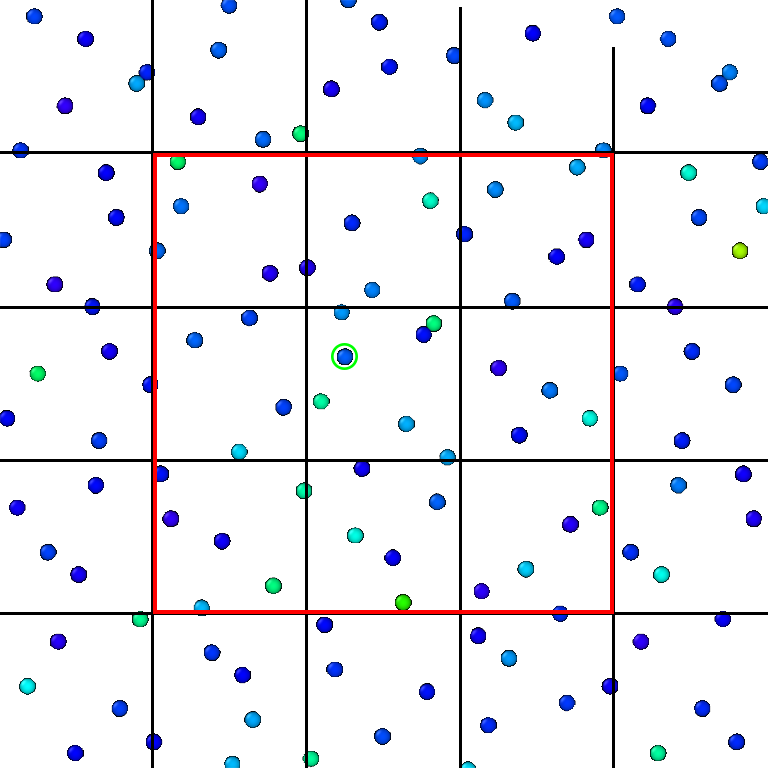
\includegraphics[height=0.5\textheight]{MD_diagram.png}
						\\\tiny MD snapshot with nearest neighbor cells
					\end{center}
				\end{column}
			\end{columns}
		\end{itemize}
	\end{frame}
	
	\begin{frame}{MD Implementation}
		\begin{itemize}
			\item  Velocity Verlet time evolution:\vspace{-0.2em}
			\small\begin{align*}
			v\left(t+\frac{\Delta t}{2}\right) &= v(t) + \frac{\Delta t}{2}\frac{F(t)}{m} \\
			x(t+\Delta t) &= x(t) + \Delta t\:v\left(t+\frac{\Delta t}{2}\right) \\
			v(t+\Delta t) &= v\left(t+\frac{\Delta t}{2}\right) + \frac{\Delta t}{2}\frac{F(t+\Delta t)}{m}
			\end{align*}\normalsize
			\item  Yukawa potential for particles $i$, $j$:\vspace{-0.2em}
			\small\begin{align*}
			V_{ij} &= \frac{Z_iZ_je^2}{4\pi\varepsilon_0r_{ij}}e^{-\frac{r_{ij}}{\lambda}} \\
			F_{ij} &= -\frac{\partial V_{ij}}{\partial r_{ij}} = V_{ij}\left(\frac{1}{r_{ij}}+\frac{1}{\lambda}\right)
			\end{align*}\normalsize
		\end{itemize}
	\let\thefootnote\relax\footnotetext{\tiny Thank you to Mathieu Marciante for the base MD code.}
	\end{frame}
	
	\begin{frame}{Deriving BGK from MD}
		\begin{itemize}
			\item  We construct a Klimontovich distribution, $N_k$, for each species that encodes the location, $\mathbf{r}_i$, and velocity, $\mathbf{v}_i$, of each ion $i$ of each species $k$ at a given time $t$:
			\begin{equation*}
				N_k(\mathbf{r},\mathbf{v},\{\mathbf{r}_\alpha\}_{\alpha=1}^{N},\{\mathbf{v}_\alpha\}_{\alpha=1}^{N},t) = \sum_{i\in S_k}\delta\left(\mathbf{r}-\mathbf{r}_i(t)\right)\delta\left(\mathbf{v}-\mathbf{v}_i(t)\right).
			\end{equation*}
			\item After defining the distribution of species $k$ as 
			\[f_1^{(k)}(\mathbf{r},\mathbf{v},t)=E[N_k],\]
			we use the Hamiltonian of the system of all species to derive a partial differential equation for $f_1^{(k)}$
		\end{itemize}
	\end{frame}
	
		\begin{frame}{Model Derivation}
		\begin{itemize}
			\item  For a general potential energy $U_{\{kl\}}$ that depends on the species of the two ions as well as their positions, this can be written as
			\begin{align*}
			\frac{\partial f_1^{(k)}}{\partial t}=&-\mathbf{v}\cdot\nabla_\mathbf{r}f_1^{(k)}\\&+\frac{1}{m_k}\nabla_\mathbf{r}\cdot\nabla_\mathbf{v}\left(\sum_l\int U_{\{kl\}}(\mathbf{r},\mathbf{r}')f_{2}^{(kl)}(\mathbf{r},\mathbf{v},\mathbf{r}',\mathbf{v}',t)\,d\mathbf{r}'\right)
			\end{align*}
			\item This defines the BBGKY hierarchy, which is still exact		
			\vspace{0.25em}
		\end{itemize}
		\begin{center}
			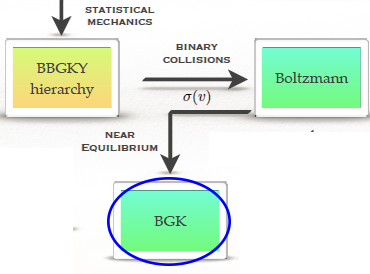
\includegraphics[height=0.3\textwidth]{KT_structure_zoom.png}
		\end{center}
	\end{frame}
	
	\begin{frame}{Model Derivation}
	\begin{itemize}
	\item The $f_2^{(kl)}$ are eight dimensional plus time, and so are very difficult to capture with a small MD simulation
	\vspace{1em}
	\begin{itemize}
	\item Instead, we use the BGK approximation:
	\[f_2^{(kl)}(\mathbf{r},\mathbf{v},\mathbf{r}',\mathbf{v}',t)=f_1^{(k)}(\mathbf{r},\mathbf{v},t)f_1^{(l)}(\mathbf{r}',\mathbf{v}',t)+C
	\]
	\end{itemize}
	\item This results in:
			\begin{align*}
				\frac{\partial f_1^{(k)}}{\partial t}=&-\mathbf{v}\cdot\nabla_\mathbf{r}f_1^{(k)}\\&+\frac{1}{m_k}\nabla_\mathbf{r}\left(\sum_l\int U_{\{kl\}}(\mathbf{r},\mathbf{r}')n_l(\mathbf{r}',t)\,d\mathbf{r}'\right)\cdot\nabla_\mathbf{v}f_1^{(k)}\\&+\sum_l\frac{f_{eq}^{(kl)}-f_1^{(k)}}{\tau_{kl}}
			\end{align*}where $n_l(\mathbf{r}',t)=\int f_1^{(l)}d\mathbf{v}$ is the ion density of species $l$
			\end{itemize}
			\end{frame}
			
			\begin{frame}{Model Derivation}
			\begin{itemize}
	\item Let $U_{\{kl\}}$ be the Yukawa potential or the Coulomb potential, and $E(\mathbf{r},t)$ be the electric field at $\mathbf{r}$ at time $t$ due to this potential. Then, this reduces to the Vlasov equation:
			\begin{equation*}
			\frac{\partial f_1^{(k)}}{\partial t}+\mathbf{v}\cdot\nabla_\mathbf{r}f_1^{(k)}+\frac{Z_k e}{m_k}E(\mathbf{r},t)\cdot\nabla_\mathbf{v} f_1^{(k)}=\sum_l\frac{f_{eq}^{(kl)}-f_1^{(k)}}{\tau_{kl}}
			\end{equation*}
			\item The electric potential for a charge distribution with the Yukawa potential is a solution to the screened Poisson equation
			\[\left(\bigtriangleup-\frac{1}{\lambda^2}\right)\phi(\mathbf{r}) = -\frac{1}{\epsilon_0}\sum_l eZ_l n_l(\mathbf{r})
			\]
			\item Solve this linear equation for $\phi$ and use $E(\mathbf{r},t)=\nabla_\mathbf{r}\phi$
\end{itemize}
	\end{frame}
	
	\begin{frame}{Kinetic Implementation}
		\begin{itemize}
			\item  We use a second order finite volume method to evolve the PDE\end{itemize}\begin{center}
			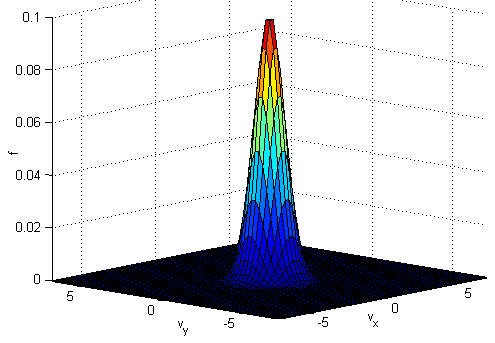
\includegraphics[height=0.3\textheight]{example_f.png}
			\\\tiny $f_1^{(k)}(\boldsymbol{v})$ at a single $x$ location
		\end{center}
			\begin{itemize}\item  Taking advantage of the symmetry we introduced from the start, we can solve a 1D PDE for the evolution
			\[\frac{\partial f_1^{(k)}}{\partial t}+v_x\frac{\partial f_1^{(k)}}{\partial x}+\frac{Z_k e}{m_k}E(x)\frac{\partial f_1^{(k)}}{\partial v_x}=\sum_l\frac{f_{eq}^{(kl)}-f_1^{(k)}}{\tau_{kl}(x)}
			\]

		\end{itemize}
	\let\thefootnote\relax\footnotetext{\tiny Thank you to Jeff Haack for the base KT code.}
	\end{frame}
	
	
	
	\begin{frame}[t]{Comparison of Models}
		\vspace{-0.8em}
		\begin{columns}
			\begin{column}{0.55\textwidth}
				\begin{center}\textbf{Molecular Dynamics}\end{center}\vspace{-0.8em}
				\begin{itemize}
					\item  \color{blue}Conserves total energy
					\item  Simulating random walk of particle interactions ``exactly''
					\item  Full particle correlations
					\item  \color{red}Noisy, need ensemble average to calculate bulk properties
					\item  Requires very small time step
					\item  \ovalbox{Computationally expensive}
				\end{itemize}
			\end{column}
			\begin{column}{0.55\textwidth}
				\begin{center}\textbf{Kinetic Theory}\end{center}\vspace{-0.8em}
				\begin{itemize}
					\item  \color{red}Only conserves kinetic energy
					\item  Simulating particle interactions in average sense
					\item  No particle correlation data
					\item  \color{blue}Can calculate bulk properties directly from $f$
					\item  Relatively large time steps
					\item  \ovalbox{Computationally inexpensive}
				\end{itemize}
			\end{column}
		\end{columns}
		\begin{center}
			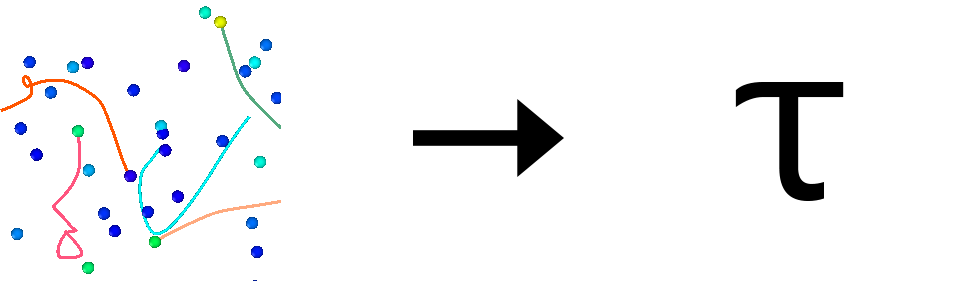
\includegraphics[height=0.3\textheight]{random_walk.png}
		\end{center}
	\end{frame}
	
	\subsection{Connecting the Models}
	\begin{frame}{Connecting the Models with $\tau$}
		\begin{itemize}
		\item BGK attempts to approximate the collisional terms of the Boltzmann equation by relaxing the distribution towards interparticle equilibria with relaxation times $\tau_{kl}$
		\vspace{0.5em}
		\item We select the $\tau_{kl}(x)$ such that relevant physical rates in BGK match observed rates in an MD simulation
		\vspace{0.5em}\begin{itemize}
		\item Rate of change of entropy density\vspace{0.5em}
		\item Rate of exchange of kinetic energy between different species\end{itemize}\vspace{0.5em}
		\item By requiring that our BGK model match the entropy production rate due to each species and the kinetic energy exchange between each species at each spatial position, we can compute approximations of $\tau_{kl}(x)$
		
		\end{itemize}
	\end{frame}
	
	
	\begin{frame}{Reconstruction (How to initialize MD from $f$)}
		\begin{itemize}
		\item Compute $\tau_{kl}$ at each macro grid point by using a much much smaller microscale simulation constrained by macroscale state
		\vspace{0.5em}
		\begin{itemize}
		\item Because $f$ is high dimensional, directly sampling it accurately would require prohibitively many particles
		\end{itemize}

		\vspace{0.5em}
		\item We use a three-step process for initializing each microcell for an MD simulation
		\vspace{0.5em}
		\begin{itemize}
		\item[1. ] Use a Halton sequence to place a set number of particles in $x$ bins to match the density of $f$ at the position
		\vspace{0.5em}
		\item[2. ] Use a Langevin thermostat to equilibrate the microcell to its proper temperature
		\vspace{0.5em}
		\item[3. ] Once properly correlated, draw new velocities for each particle from the velocity distribution at that $x$ position
		\end{itemize}
		\end{itemize}
	\end{frame}
	

	
	\begin{frame}{Reconstruction (Velocity Resample)}
		\begin{itemize}
			\item Interpolate the velocity distribution for each bin so it is not ``too discrete''
			\vspace{1em}
			\item Assign particle velocities to particles in each bin by sampling the 2D probability distribution function
			\vspace{1em}
			\item Our velocity resampling algorithm accurately captures at least the first three moments of the velocity distribution with sufficient particles
			\vspace{1em}
			\item \emph{Question}: How important are the velocity correlations that we are throwing out?
		\end{itemize}
	\end{frame}
	
	
		\begin{frame}{Computing Statistics}
		\begin{itemize}
			\item Once the MD simulation is running, we record data
			\vspace{1em}
			\item Averaging over time gives an approximate ensemble average of the different rates of change
			\vspace{1em}
			\begin{itemize}
			\item Not yet implemented --- how noisy will the statistics be?
			\end{itemize}
			\vspace{1em}
			\item These averages are then used to directly compute $\tau_{kl}$ such that the BGK will have these same rates of change
		\end{itemize}
	\end{frame}
	
	\section{Summary}
	\begin{frame}{Summary}
		\begin{itemize}
			\item HMM provides a framework to provide hybrid multiphysics simulations that combine the accuracy of the microscale with the efficiency of the macroscale
			\vspace{1em}
			\item Extra attention must be paid to the connection between the two models (compression and reconstruction)
			\vspace{1em}
			\item We have the theoretical framework to model plasmas using kinetic theory and molecular dynamics
			\vspace{1em}
			\begin{itemize}
			\item My collaborators in Los Alamos and I are continuing work on this project
			\end{itemize}
		\end{itemize}
	\end{frame}
	




	
	\section{Future Work}
	\begin{frame}{Future Work}
		\begin{itemize}
			\item Implement model in Python to improve efficiency
			\begin{itemize}
			\vspace{0.5em}
			\item Run bevy of stress tests of each method separately
			\vspace{0.5em}
			\item Implement the explicit connection for a working HMM model
			\vspace{0.5em}
			\item Apply to relevant real world problems for publication\vspace{0.5em}
			\end{itemize}
			\item Conduct numerical and statistical analysis of various aspects of the method, potentially finding error bounds\vspace{0.5em}
			\item Validate model with experimental results
			\vspace{0.5em}
			\item Apply HMM to other applications with similar robust analysis
		\end{itemize}
	\end{frame}

	

	
	
	
\end{document}